\documentclass[../monografia.tex]{subfiles}

\graphicspath{ {images/}{../images/} }

\begin{document}


Para o desenvolvimento do projeto, dividimos as tarefas entre 3 áreas: Hardware, Firmware e Software. 

No \textbf{hardware} estará concentrado todo o desenvolvimento da eletrônica dos dispositivos que estarão nos nós da rede. 
O \textbf{firmware} será todo o software embarcado no dispositivo, desde a comunicação com o hardware até a comunicação sem fio, entre os dispositivos da rede e do dispositivo \textit{gateway} com a plataforma. 
O \textbf{software}, por fim, trata do desenvolvimento relacionado à plataforma onde os dados serão armazenados e apresentados. 

Por fim, foi desenvolvido um case mecânico simples, impresso em 3D, para proteger os componentes. 

\section{Hardware}

A partir das especificações técnicas, foi elaborado um novo diagrama de blocos. 

\begin{figure}[h]
    \centering
    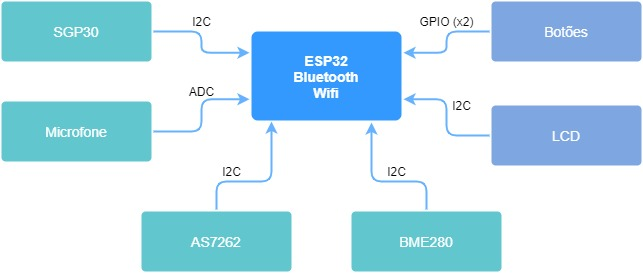
\includegraphics[width=12cm]{diagrama_hw_v1}
    \caption{Diagrama de Blocos de Hardware do Protótipo}
    \label{fig:img1}
\end{figure}

Quando possível, foram utilizados kits de desenvolvimento e módulos que nos permitisse uma validação mais rápida do hardware nessa fase inicial, permitindo avançar mais com o firmware e fazer testes em campo. 

O DevKitC do ESP32 possui integrado um USB, através do qual é possível alimentar os demais subcircuitos da placa, não existindo a necessidade de uso de bateria nessa etapa. 

\subsection{Esquemático}

Para o design do hardware, utilizamos o software de CAD de PCB \textit{Altium Designer 20} \cite{altium}. Foi utilizada a licença da empresa orientadora, sendo possível também conseguir uma licença gratuita para estudantes. Os arquivos estão disponíveis em \cite{git_hw}. 

A partir do diagrama de blocos, foi desenvolvido o esquema elétrico

\begin{figure}[h]
	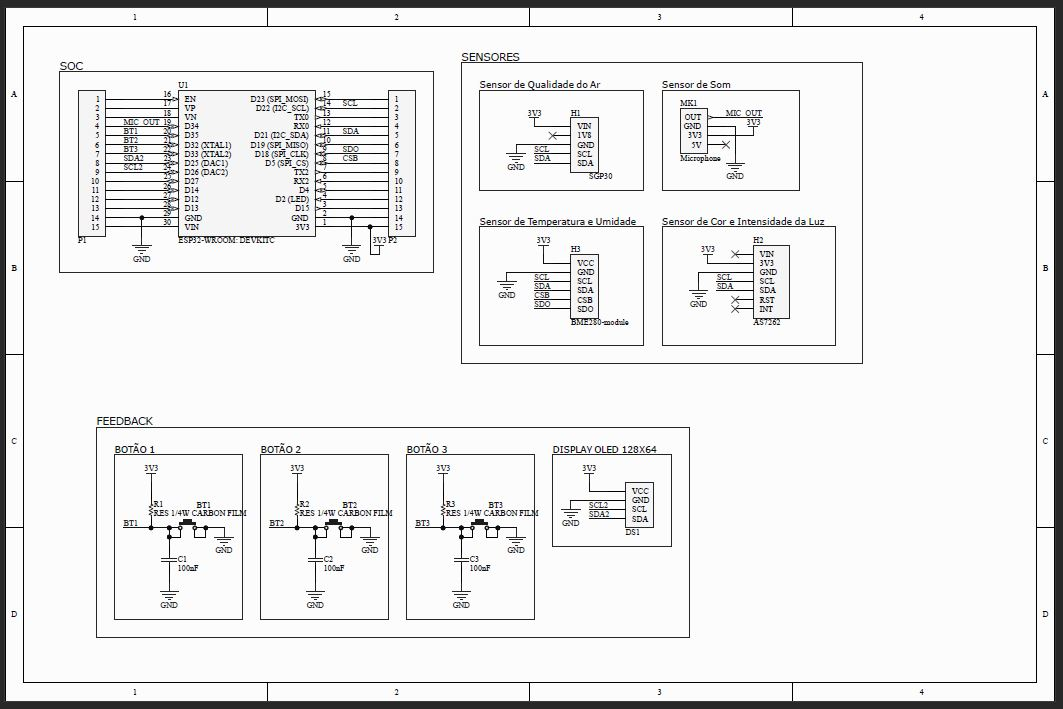
\includegraphics[width=0.9\textwidth]{sch}
	\caption{Esquemático do Protótipo}
	\label{fig:img2}
\end{figure}

\subsection{PCB \textit{Printed Circuit Board}}

A partir do esquema elétrico foi feito um desenho de PCB (\textit{Printed Circuit Board}, ou Placa de Circuito Impresso), \textit{Single Layer}, e dimensões finais 60x70mm. 

\begin{figure}[ht]
	\centering
	\begin{subfigure}{0.5\textwidth}
	  \centering
	  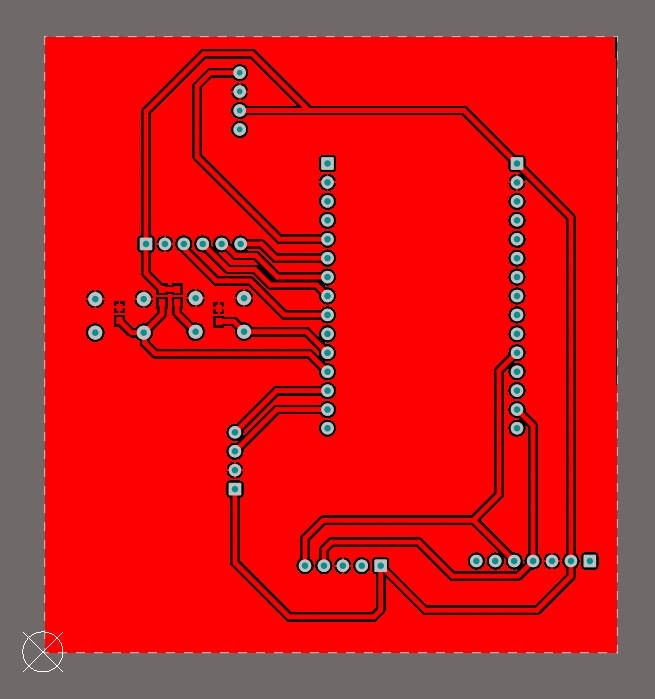
\includegraphics[width=.7\linewidth]{pcb_2}
	  \caption{Vista 2D}
	  \label{fig:sub1}
	\end{subfigure}%
	\begin{subfigure}{0.5\textwidth}
	  \centering
	  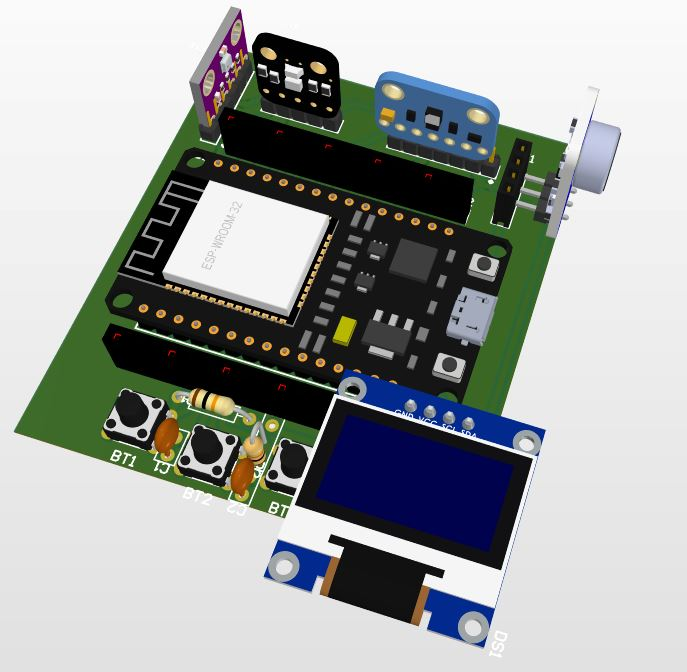
\includegraphics[width=.9\linewidth]{hw-3d}
	  \caption{Vista 3D}
	  \label{fig:sub2}
	\end{subfigure}
	\caption{Design da PCB}
	\label{fig:test}
\end{figure}

As placas foram fabricadas em fibra por uma fresadora CNC.

\begin{figure}[h]
	\centering
	\begin{subfigure}{0.5\textwidth}
		\centering
		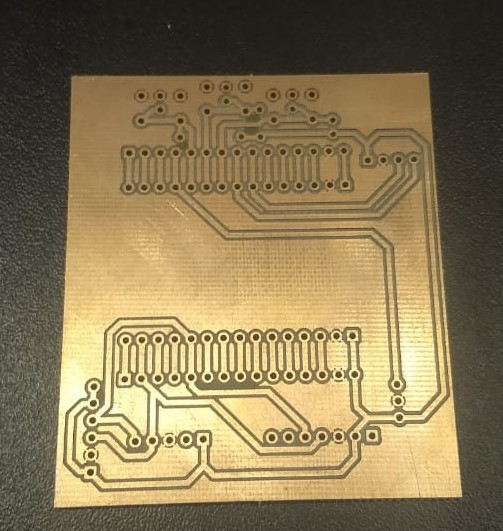
\includegraphics[width=0.8\textwidth]{pcb-fresada}
	\end{subfigure}%
	\begin{subfigure}{0.5\textwidth}
		\centering
		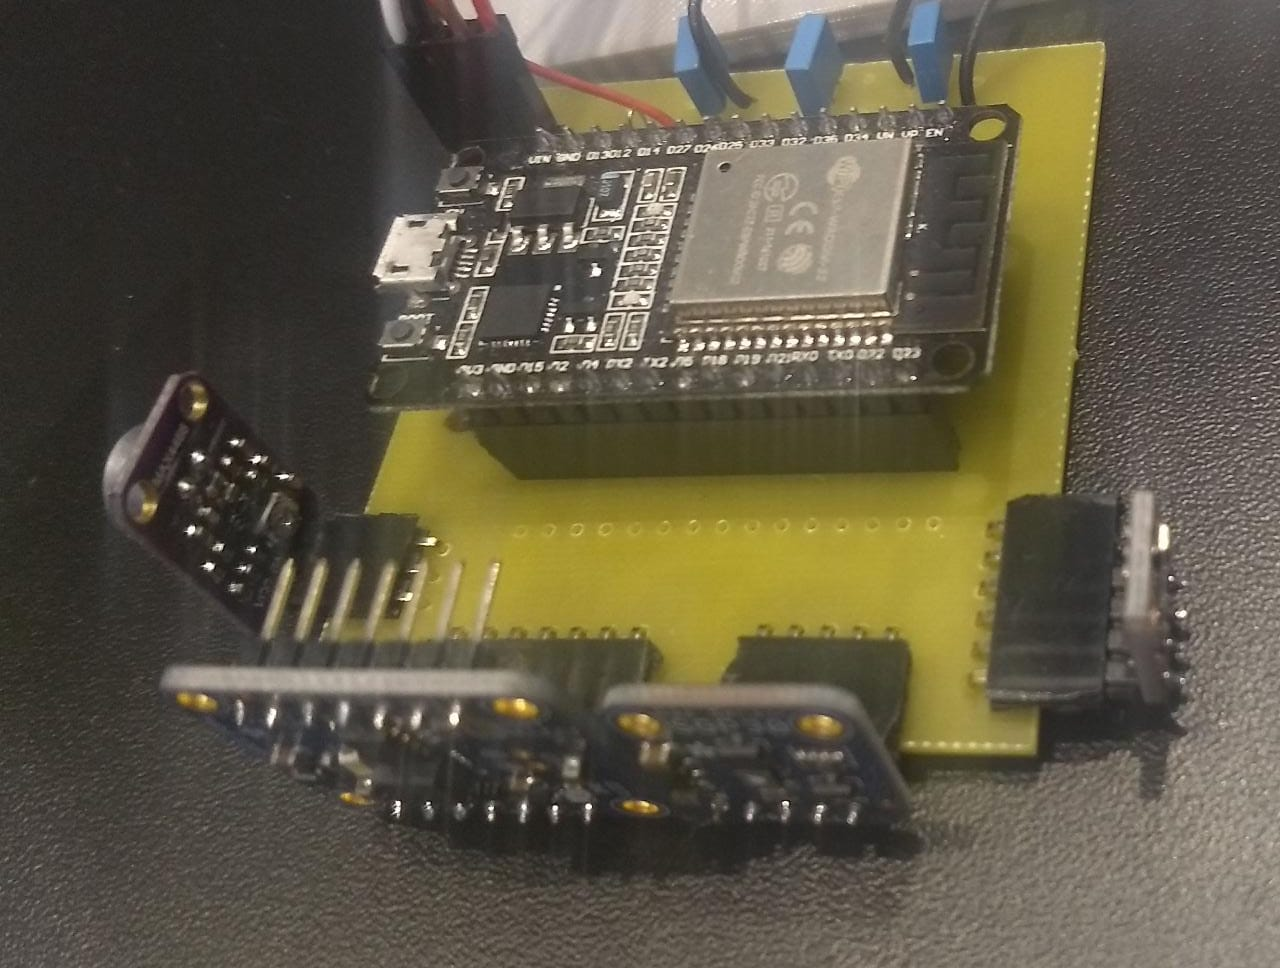
\includegraphics[width=1.1\textwidth]{pcb-montada}
	\end{subfigure}
	\caption{PCB}
	\label{fig:mecanicas}
\end{figure}


\section{Firmware} \label{firmware}

O desenvolvimento do firmware se deu utilizando o \textbf{ESP-IDF} (\textit{Espressif IoT Development Framework}), disponível pela Espressif\cite{esp-idf} gratuitamente (sob \textit{Apache License}). 

O ESP-IDF é composto por API, ferramentas, componentes e fluxos de trabalho (\textit{workflows}) que permitem o desenvolvimento de aplicações utilizando o ESP32. 

Além disso, utiliza o FreeRTOS, que é o principal sistema operacional de tempo real (RTOS) para microcontroladores\cite{freertos}, de código aberto (\textit{MIT open source license}), e com suporte para diversas famílias de microcontroladores.

Como o ESP32 possui 2 Cores, o FreeRTOS usado no IDF é uma versão modificada do \textit{vanilla} FreeRTOS, permitindo que exista multiprocessamento simétrico (SMP, \textit{symmetric multiprocessing}).

Outras bibliotecas, proprietárias ou disponíveis em código aberto, foram utilizadas para a integração de todos os periféricos. 

A camada mais alta do software nos dispositivos, separamos em três: sensores, feedback e rede; descritas a seguir. %??

\begin{figure}[h!]
	\centering
	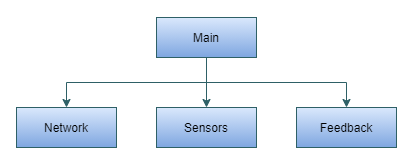
\includegraphics[scale=0.8]{fw-arch-1}
	\caption{Camada alto nível do firmware dos dispositivos}
	\label{fig:fw-arch}
\end{figure}

A arquitetura completa do firmware está disposível no Anexo 2. %???

\subsection{Sensores} %\label{sensores}

Para os sensores, desenvolvemos bibliotecas baseadas no ESP-IDF e validamos o funcionamento dos mesmos individualmente realizando algumas coletas de dados do ambiente. 

\begin{figure}[h]
	\centering
	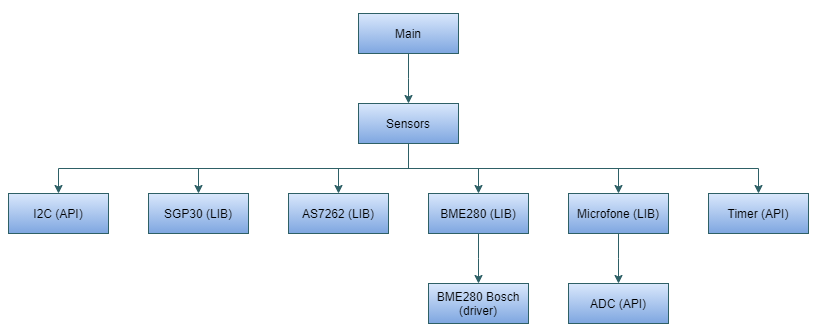
\includegraphics[width=0.9\textwidth]{sensors-arch}
	\caption{Arquitetura dos Sensores}
	\label{fig:sensors-arch}
\end{figure}

\subsubsection{BME280}

O BME280 é um sensor da Bosch que realiza medições de temperatura, umidade e pressão no ambiente. Possui 3 modos de operação: \cite{bme280}
\begin{itemize}
	\item \textit{sleep}: baixo consumo de energia, registradores podem ser lidos mas não realiza novas operações de medição.
	\item \textit{forced}: realiza uma medição, salva os resultados, e volta ao modo \textit{sleep}.
	
	\begin{figure}[h]
		\centering
		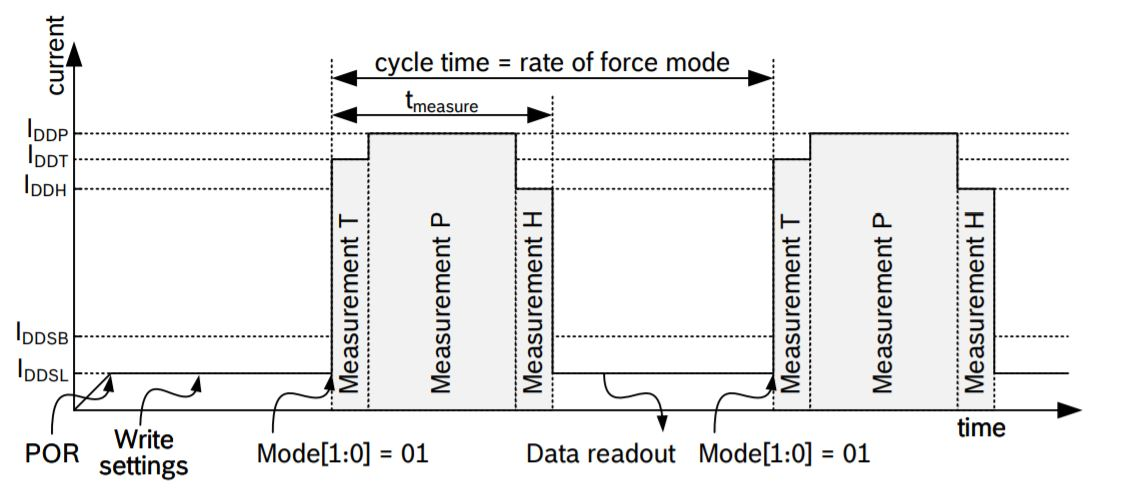
\includegraphics[width=12cm]{timing_bme280}
		\caption{Diagrama de tempos do modo \textit{forced}}
		\label{fig:time_bme280}
	\end{figure}

	\item normal: realiza medições periodicamente. O consumo durante o \textit{standby} entre medições é maior que o consumo no modo \textit{sleep}. 
\end{itemize}

O \textit{datasheet} recomenda que, para aplicações do tipo \textbf{monitoramento climático}, seja utilizado o modo \textit{forced}, com cerca de 1 medição por minuto. Assim, o sensor consumirá uma corrente de aproximadamente 0.16$\mu$A, sendo o modo de maior economia de energia. 

A Bosch Sensortech disponibiliza um driver para o BME280, com código fonte em C e disponibilizado abertamente\cite{bme280-driver}, que permite sua integração ao firmware em microcontroladores de qualquer fabricante. 
Utilizando o driver como base, desenvolvemos uma biblioteca para a utilização do BME280 no ambiente ESP-IDF, utilizando comunicação I2C, disponível

%todo: colocar estrutura da lib

%* Teste de validação 
%? manter?
% \begin{figure}[h]
% 	\centering
% 	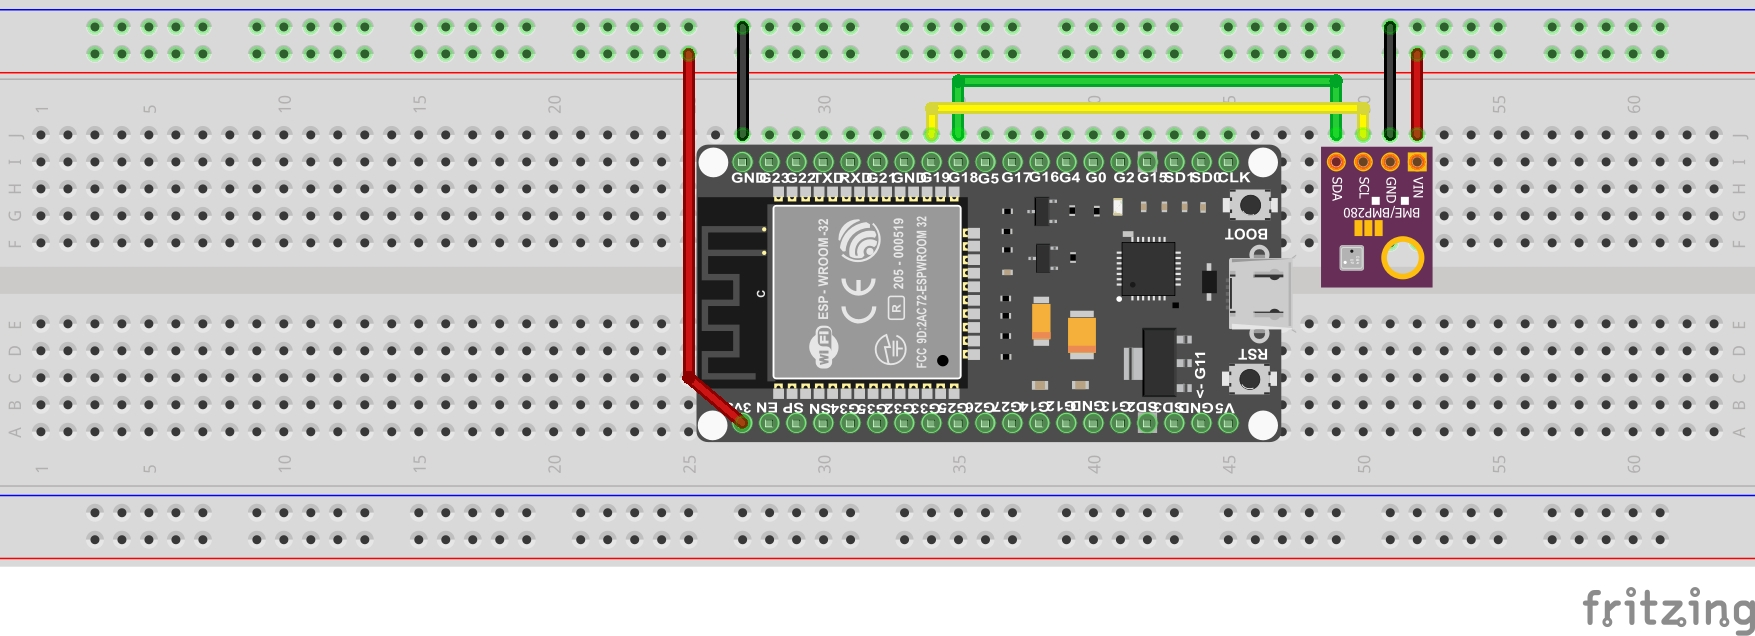
\includegraphics[width=12cm]{teste_bme280}
% 	\caption{Montagem na Protoboard do Teste com o sensor BME280}
% 	\label{fig:time_bme280}
% \end{figure}

\subsubsection{AS7262}

Para a medição de parâmetros relacionados a luminosidade, foi utilizado o sensor AS7262, da AMS, que possui filtros internos capazes de separar a luz visível de acordo com 6 comprimentos de onda: 450, 500, 550, 570, 600 e 650 nm - que correspondem às cores violeta, azul, verde, amarela, laranja e verde, respectivamente. Cada um dos filtros é lido por conversores analógico-digital de 16 bits de resolução independentes que salvam os dados em registradores internos a cada conversão realizada. Possui 4 modos de operação:

\begin{itemize}
	\item \textbf{Modo 0:} realiza medições contínuas, disponibilizando dados apenas referentes às cores violeta, azul, verde e amarela, sendo que os registradores de dados das cores vemelha e laranja ficarão com valor nulo.
	\item \textbf{Modo 1:} realiza medições contínuas, disponibilizando dados apenas referentes às cores verde, amarela, laranja e vermelha, sendo que os registradores de dados das cores violeta e azul ficarão com valor nulo.
	\item \textbf{Modo 2:} realiza medições contínuas para todos os canais.
	\item \textbf{Modo 3:} realiza medições para todos os canais, porém no modo \textit{One-Shot}.
\end{itemize}

A diferença entre os modos contínuos e o modo \textit{One-Shot} é que, no segundo, o usuário controla quando as medições deverão ser realizadas, enquanto que no modo contínuo as medições são realizadas automaticamente a partir da sua inicialização.

Outra configuração disponível para que o usuário escolha é o ganho que será aplicado nos canais de leitura, podendo ser escolhido dentre os valores 1x, 3.7x, 16x e 64x.

A interface com o sensor pode ser feita através dos protocolos I²C, utilizada nesse projeto, ou UART, através de comandos AT. Foi desenvolvida uma biblioteca na linguagem C no formato adequado para ser utilizada no ESP-IDF com a implementação das principais funções do sensor. Ao acessar o barramento I²C, só será possível visualizar 4 endereços de registradores físicos, de acordo com a tabela ~\ref{table:as7262-registers-table}.

% Please add the following required packages to your document preamble:
% \usepackage[table,xcdraw]{xcolor}
% If you use beamer only pass "xcolor=table" option, i.e. \documentclass[xcolor=table]{beamer}
\begin{table}[htp]
\begin{tabular}{|c|c|l|ll}
\cline{1-3}
\cellcolor[HTML]{C0C0C0}\textbf{Registrador} & \cellcolor[HTML]{C0C0C0}\textbf{Descrição} & \multicolumn{1}{c|}{\cellcolor[HTML]{C0C0C0}\textbf{Nota}}                                                                         &  &  \\ \cline{1-3}
\textit{Device Slave Address}                & Endereço I²C de 8 bits                     & \begin{tabular}[c]{@{}l@{}}Endereço = 1001001x (0x49), onde\\   x = 1 representa leitura\\   x = 0 representa escrita\end{tabular} &  &  \\ \cline{1-3}
STATUS                                       & Registrador de STATUS                      & \begin{tabular}[c]{@{}l@{}}Endereço 0x00\\ Sinaliza se os registradores de Leitura\\ e Escrita estão disponíveis\end{tabular}      &  &  \\ \cline{1-3}
WRITE                                        & Registrador de Escrita I²C                 & \begin{tabular}[c]{@{}l@{}}Endereço 0x01\\ \\ Valor de 8 bits a ser escrito pelo Mestre\end{tabular}                               &  &  \\ \cline{1-3}
READ                                         & Registrador de Leitura I²C                 & \begin{tabular}[c]{@{}l@{}}Endereço 0x02\\ \\ Valor de 8 bits a ser lido pelo Mestre\end{tabular}                                  &  &  \\ \cline{1-3}
\end{tabular}
\caption{Registradores físicos do sensor AS7262}
\label{table:as7262-registers-table}
\end{table}

O endereçamento dos registradores de aplicação, como os que armazenarão os dados coletados e modos de operação se dá de modo virtual. O \textit{datasheet} descreve a lógica de leitura e escrita nesses registradores virtuais:

\begin{itemize}
\item Escrita em Registrador Virtual:
	\begin{itemize}
		\item Primeiramente, ler o valor do registrador STATUS;
		\item Se o bit 1 desse registrador for igual a 0, significa que a escrita pode ser realizada;
		\item Escrever o endereço do registrador virtual no registrador WRITE (0x01) com o \textbf{MSB igual a 1} para indicar que será realizada uma escrita nele;
		\item Ler novamente o valor do registrador STATUS e verificar se o bit 1 é igual a 0;
		\item Finalmente, escrever o valor desejado para o registrador virtual no registrador WRITE.
	\end{itemize}
	
\item Leitura em Registrador Virtual:
	\begin{itemize}
		\item Primeiramente, ler o valor do registrador STATUS;
		\item Se o bit 1 desse registrador for igual a 0, significa que a escrita pode ser realizada;
		\item Escrever o endereço do registrador virtual no registrador WRITE (0x01) com o \textbf{MSB igual a 0} para indicar que será realizada uma leitura de seu valor;
		\item Ler o valor do registrador STATUS e verificar se o bit 0 é igual a 1, indicando que os dados estão prontos para serem lidos;
		\item Finalmente, ler o registrador READ (0x02), que estará com os dados requisitados.
	\end{itemize}
\end{itemize}

A lista com todos os endereços dos registradores virutais pode ser encontrada em seu \textit{datasheet} \cite{as7262}. Com essas rotinas de leitura e escrita implementadas, basta realizar a configuração desejada para a aplicação e depois ler os valores captados pelo sensor. 

\begin{figure}[h]
	\centering
	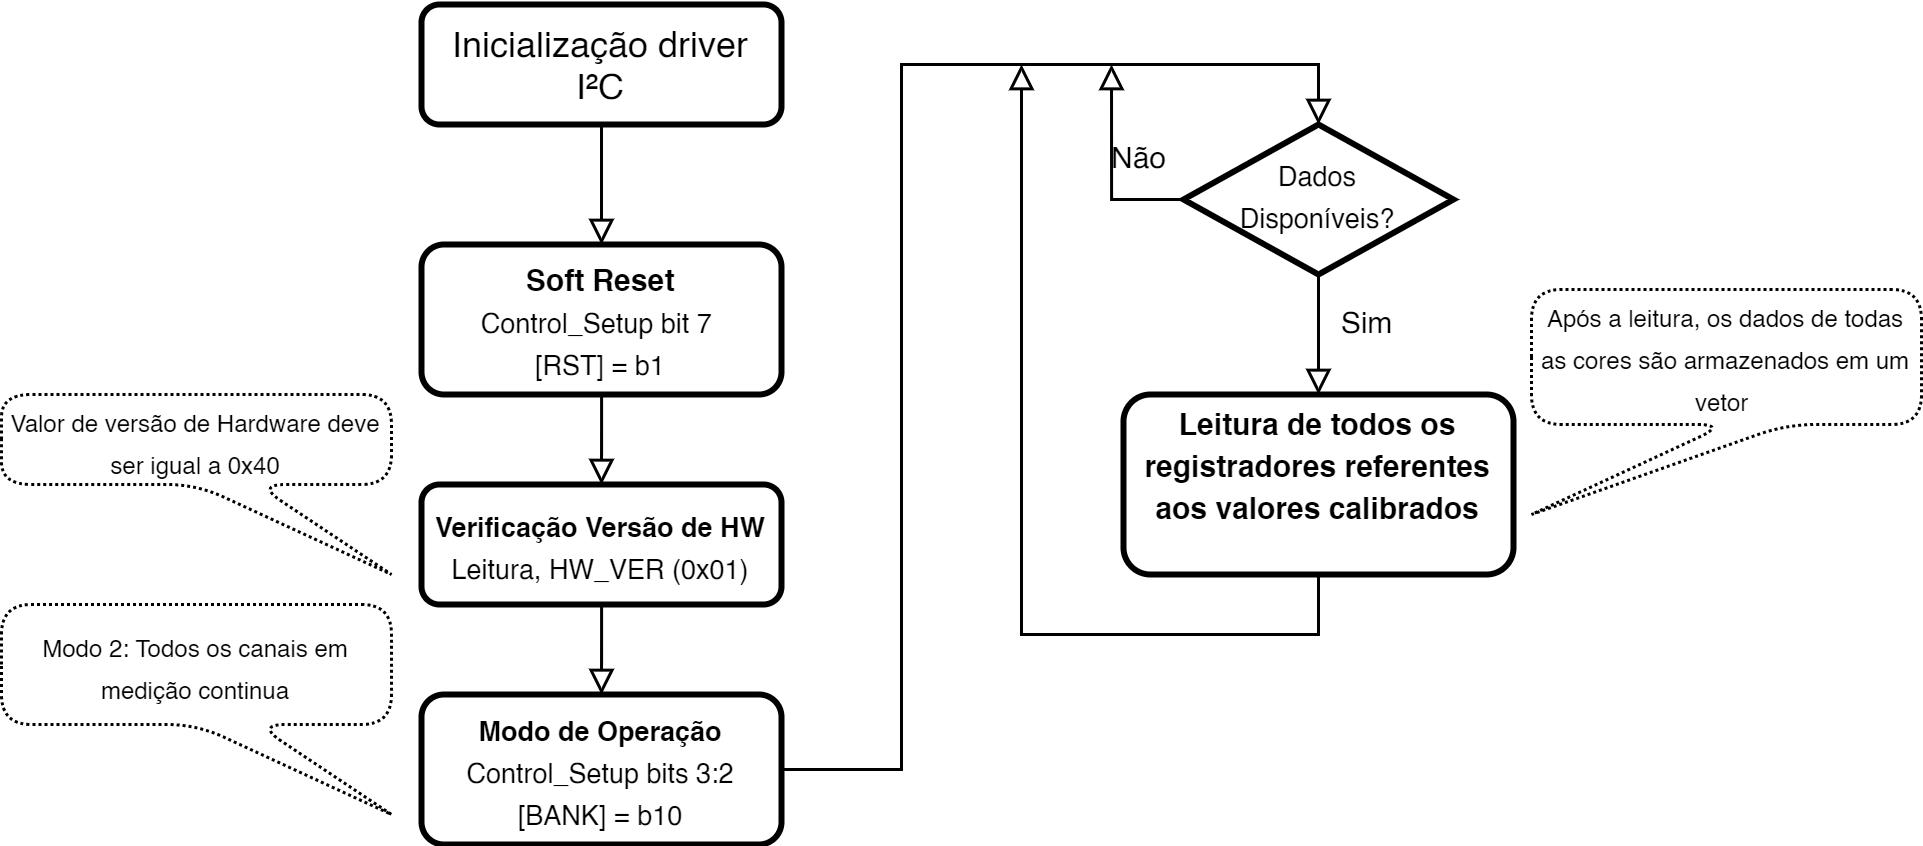
\includegraphics[scale=0.2]{as7262_firmware.png}
	\caption{Fluxograma da lógica de firmware para operação do sensor AS7262}
	\label{fig:as7262_firmware}
\end{figure}

A figura \ref{fig:as7262_firmware} mostra a lógica de aplicação implementada neste projeto. Primeiramente, é feita a operação de \textit{Soft Reset} no sensor para reinicializá-lo, depois é feita a verificação do registrador que indica a versão do Hardware, que deve ser igual a 0x40. Feita essa verificação, escreve-se o valor 0b10 para inicializar a captação de valores no \textbf{Modo 2}: modo contínuo, referentes a todos os canais de medição. O valor de cada canal será armazenado em 4 registradores, totalizando 32 bits de valores em notação de ponto flutuante para cada canal. A etapa final da aplicação é realizar a leitura desses 24 registradores (4 por canal, 6 canais no total) e salvá-los em um vetor de 6 posições, para que possam ser manipulados posteriormente.

A bilbioteca desenvolvida para a interação com o sensor pode ser acessada em \cite{as7262-lib}.

%!!!!!!!!!!!!!!!! Precisa escrever sobre interpretação dos dados


\subsubsection{SGP30}

O sensor utilizado para medições dos parâmetros referentes à qualidade do ar foi o SGP30, da Sensirion. A partir de medições de concentracão de hidrogênio e etanol no ar, um algoritmo interno ao sensor consegue estimar o total de componente orgânico volátil (TVOC), em partes por bilhão (ppb), e o equivalete de $CO_{2}$, em partes por milhão (ppm), presentes no ambiente. 

A interface com esse sensor também é feita através do protocolo I²C, porém através de comandos pré-definidos, presentes nas páginas 9 e 10 do \textit{datasheet} \cite{sgp30}. Cada comando é identificado por um valor de 16 bits e é responsável por realizar uma ação no sistema, como inicializar, realizar medições e ler valores fixados, como número de série. 

Todos os dados enviados e recebidos pelo sensor contém ao final, além dos valores padrão, 8 bits de valores para verificação cíclica de redundância (do inglês \textit{Cyclic Redundancy Check}, CRC), com a finalidade de validar os dados sendo transmitidos, utilizando o método de \textit{checksum}, calculado com o seguinte polinômio: $CRC = 0h31 (x_{8} + x_{5} + x_{4} + 1)$ - em que $x_{i}$ corresponde ao i-ésimo bit do valor utilizado para o cálculo. Os comandos de 16 bits tabelados já incluem os campos do CRC em sua composição, não sendo necessário calculá-los.

Portanto, para realizar interações com o sensor, o usuário deve realizar os seguintes passos:

\begin{itemize}
	\item Inicializar a comunicação I²C com o sensor, que possui endereço 0x58, indicando ação de escrita;
	\item Enviar o valor referente ao comando que deseja ser executado (normalmente valores de 16 bits);
	\item Alguns comandos realizam respostas, como o comando \textit{Measure\_air\_quality} (0x2008). Se o comando realizado for desse tipo, basta reiniciar a comunicação I²C, agora indicando uma ação de leitura para o endereço 0x58, que os dados requisitados estarão disponíveis;
	\item Os dados de reposta virão com 8 bits de CRC ao final. O usuário pode fazer a checagem desse valor, calculando o CRC de acordo com os valores da resposta para validar os dados lidos.
\end{itemize}


Para realizar a interação com esse sensor e obter os dados necessários para esse projeto, também desenvolvemos uma biblioteca nos mesmos moldes do ESP-IDF, em linguagem C, disponível em \cite{sgp30-lib}. A rotina principal de coleta de dados é exemplificada na figura \ref{fig:sgp30_firmware}. O \textit{datasheet} indica que, para a correta inicialização do algoritmo que calcula as estimativas de $eCO_{2}$ e TVOC, é necessário que o usuário realize 14 medições espaçadas de 1 segundo, nas quais o sensor retornará valores fixos de $TVOC = 0$ e $eCO_{2} = 400 ppm$. Após esse período, o sensor começará a responder com valores válidos referentes ao ambiente em questão.

\begin{figure}[h]
	\centering
	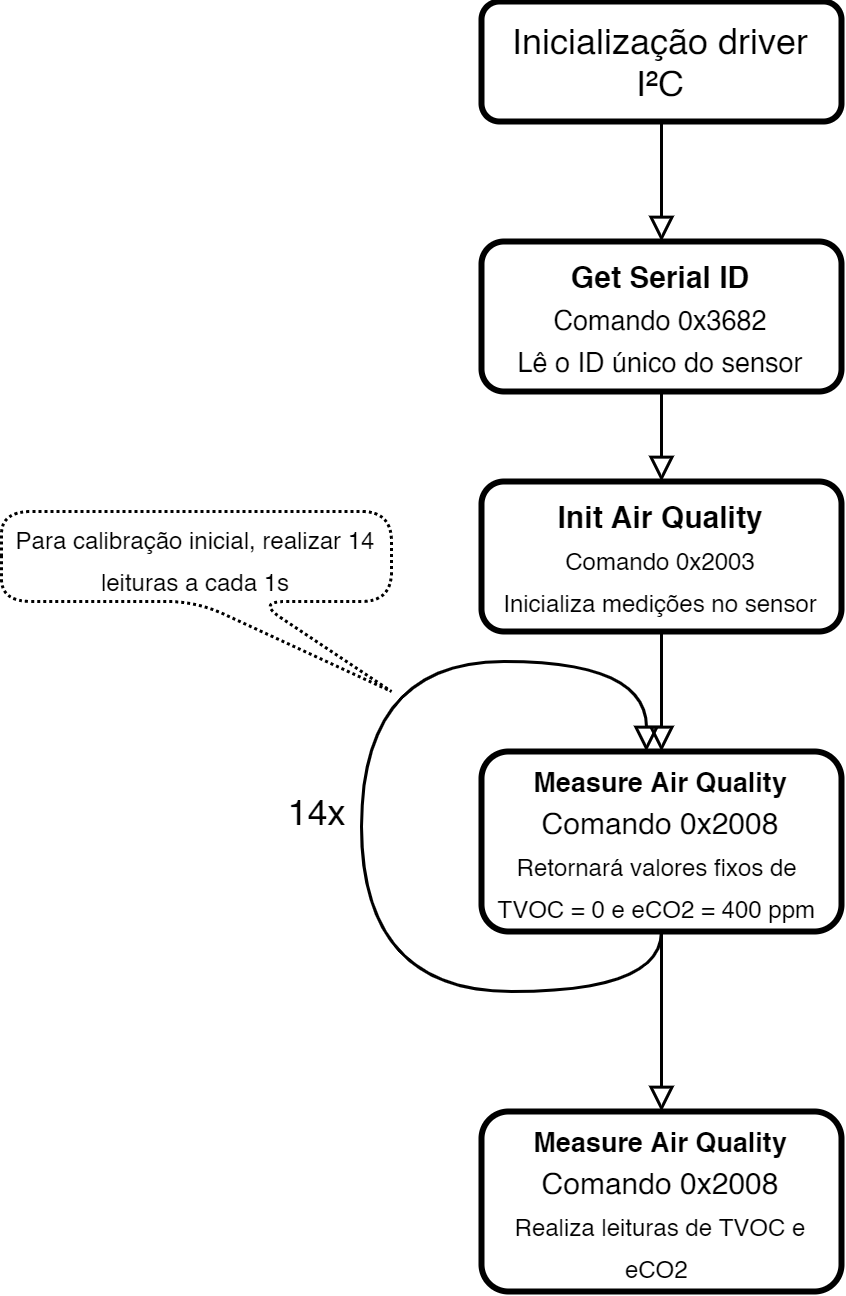
\includegraphics[scale=0.2]{sgp30_firmware.png}
	\caption{Lógica de execução de firmware para coleta de dados do sensor SGP30}
	\label{fig:sgp30_firmware}
\end{figure}

Os valores retornados pelo comando \textit{Measure Air Quality} são salvos em duas variáveis de 16 bits, a serem manipulados posteriormente.

\subsubsection{Microfone}

Para a medição de um indicador acústico, utilizamos um módulo com microfone de eletreto e um amplificador MAX4466, com ganho ajustável, da Adafruit \cite{max4466}.
A sua resposta é um sinal analógico entre 0 e 3,3V, correspondente ao sinal de áudio no ambiente, variando em torno do seu valor médio (1,65V). 

A interface com o ESP32 deu-se através do conversor analógico digital (ADC) do próprio microcontrolador. Este ADC possui uma resolução máxima de 
bits e uma amostragem máxima de 6kHz. 

\subsection{Feedback}

\begin{figure}[h]
	\centering
	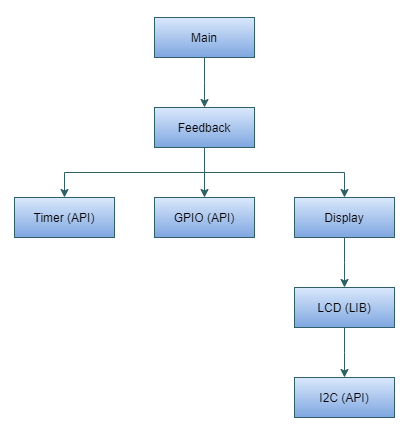
\includegraphics[scale=0.8]{feedback-arch}
	\caption{Arquitetura do Feedback}
	\label{fig:feedback-arch}
\end{figure}

A task de feedback inicialmente espera por um evento do tipo timer ser colocado na queue, identificando que deve ser realizada a coleta.

A rotina de coleta segue uma \textbf{máquina de estados}, que foi implementada a seguinte máquina de estados, seguindo um \textit{table-driven approach}.

%Máquina de Estados
\begin{figure}[h]
	\centering
	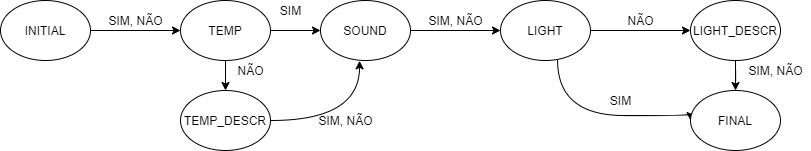
\includegraphics[width=0.9\textwidth]{fsm-feedback.png}
	\caption{Máquina de Estados da coleta de Feedback}
	\label{fig:fsm-feedback}
\end{figure}

No início de uma coleta, é executado o estado inicial e a task volta a esperar por um novo evento, que pode ser causado por um timer ou um GPIO. Caso seja um GPIO, um novo estado é executado; caso seja um timer, e o seu ID é o de Timeout, a coleta é encerrada.

A mudança entre os estados acontece quando um dos botões laterais, correspondendo a respostas 'Não' e 'Sim', é apertado. De acordo com a resposta o futuro estado é definido. 

No estado INITIAL mostra-se a primeira pergunta no display, a estrutura com as respostas é zerada e um timer TIMEOUT é iniciado, a fim de desligar a tela e encerrar o feedback caso não haja resposta. 

Em cada um dos estados intermediários, a resposta dos botões é armazenada, a tela do display é atualizada para uma nova pergunta, e o timer TIMEOUT é reiniciado. 

Quando ocorre um timeout, é executando o estado FINAL. 

%Display
O display utiliza uma porta I2C diferente dos sensores, para ter maior independência entre as tasks.

Como biblioteca para o display SSD1306, utilizamos um componente desenvolvido por Tara K\cite{TaraK} baseado no ESP-IDF\cite{SSD1306}. Em \textit{display.c} desenvolvemos as telas a serem utilizadas durante a rotina de coleta de feedback. 

%? estrutura do código

\subsection{Conectividade}

O módulo que trata da parte de rede do dispositivo foi separado em 2 partes, como exemplificado na figura \ref{fig:netw-arch}: implementação dos modelos que definem a rede BLE Mesh, presente em todos os dispositivos, e a implementação da conexão com o MQTT Broker presente no servidor externo através do protocolo Wi-Fi, presente apenas no dispositivo gateway.

\begin{figure}[h!]
	\centering
	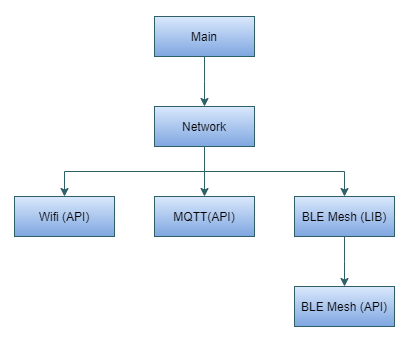
\includegraphics[scale=0.8]{netw-arch}
	\caption{Arquitetura do módulo de Conectividade} %nome feio kk
	\label{fig:netw-arch}
\end{figure}

\subsubsection{Bluetooth} \label{dev-bluetooth-section}

Como citado em seções anteriores, os dispositivos desse projeto foram interconectados em uma rede BLE Mesh para que os dados coletados por eles sejam enviados pela rede para um dispositivo com função de \textit{gateway}. Para realizar a implemenação da rede, foi utilizada a biblioteca ESP-BLE-MESH, da Espressif, sendo essa baseada na biblioteca de Bluetooth Mesh do \textit{Zephyr Project} \cite{zephyrproject}, um projeto de RTOS mantido pela \textit{Linux Foundation}, que disponibiliza toda a API necessária para a implementação de uma rede BLE Mesh customizada.

Por se tratar de uma aplicação com vários dados de sensores para serem enviados, foi criado um Modelo customizado que engloba todos os dados dos sensores que compõem um dispositivo, chamado de \textit{\textbf{Custom Sensor Model}}, o qual foi implementado tanto o Modelo Cliente quanto o Servidor. A estrutura de dados principal que define o estado do Modelo contém as seguintes variáveis: 

% !!!!!!!!!!!!!!!!! COLOCAR A ESTRUTURA DE DADOS DO BLE MESH AQUI !!!!!!!!!!!!!!!!
\begin{lstlisting}[basicstyle=\tiny,language=C,]
	typedef struct __attribute__((packed)) {
		char device_name[6];
		
		/**< BME280 Data */
		float temperature;      /*!< BME260 calibrated temperature */
		float pressure;         /*!< BME260 calibrated pressure */
		float humidity;         /*!< BME260 calibrated humidity */
	
		/**< SGP30 Data */
		uint16_t tVOC;          /*!< SGP30 total volatile organic compound */
		uint16_t eCO2;          /*!< SGP30 equivalent CO2 */
	
		/**< Mic Noise */
		uint16_t noise_level;   /*!< Analog microphone noise level */
	
		/**< AS7262 data */
		float red;              /*!< AS7262 calibrated red */
		float orange;           /*!< AS7262 calibrated orange */
		float yellow;           /*!< AS7262 calibrated yellow */
		float green;            /*!< AS7262 calibrated green */
		float blue;             /*!< AS7262 calibrated blue */
		float violet;           /*!< AS7262 calibrated violet */
	
		/**< Feedback answers */
		uint8_t feedback;       /*!< Each bit corresponds to an answer */
	} model_sensor_data_t; 
\end{lstlisting}

A definição de um Modelo também requer que sejam definidas as mensagens utilizadas para interação, sendo elas:

\begin{itemize}
	\item \textbf{GET}: mensagem utilizada para requisitar o estado atual do Modelo. Ao receber essa mensagem, o nó deve responder a requisição com uma mensagem de STATUS. O corpo dessa mensagem pode ser enviado vazio, ou seja, apenas o endereço de destino precisa ser especificado.
	\item \textbf{SET}: mensagem utilizada para alterar o estado atual do Modelo Servidor por um agente externo (Cliente ou outro nó Servidor). Essa mensagem foi implementada sem que haja ACK, ou seja, não é enviada uma confirmação ao dispositivo transmissor que a mensagem foi recebida. Deve ser especificado o endereço de destino, seja um endereço de um elemento único ou um endereço de grupo da rede para publicar a mensagem, e o conteúdo deve conter os valores que serão atualizados no destino, de acordo com a estrutura anterior.
	\item \textbf{STATUS}: mensagem utilizada para notificar o estado atual do Modelo, normalmente enviada após receber uma mensagem do tipo GET. O conteúdo da mensagem será composto pela estrutura mostrada anteriormente.
\end{itemize}

Todos os dispositivos possuem as mesmas funcionalidades de coleta de dados de sensores, porém apenas um deles é responsável por também receber as medições de todos os outros, de modo que podemos separar os dispositivos em duas categorias diferentes: os dispositivos normais, chamados de \textit{Sensor Nodes}, e o dispositivo central, chamado de \textit{Gateway Node}. A composição lógica desses dois tipos de dispositivos está demonstrada na figura \ref{fig:mesh-node-architecture}, sendo compostos por apenas um Elemento cada, com o \textit{Configuration Server Model}, mandatório para esse tipo de dispositivo, já que é ele que exerce o papel de interlocutor com o dispositivo provisionador para que haja a atribuição das chaves NetKey e AppKey. Como pode ser observado na mesma imagem, os \textit{Sensor Nodes} possuem o \textit{Custom Sensor \textbf{Client} Model} e o dispositivo central possui o \textit{Custom Sensor \textbf{Server} Model}.

\begin{figure}[h!]
	\centering
	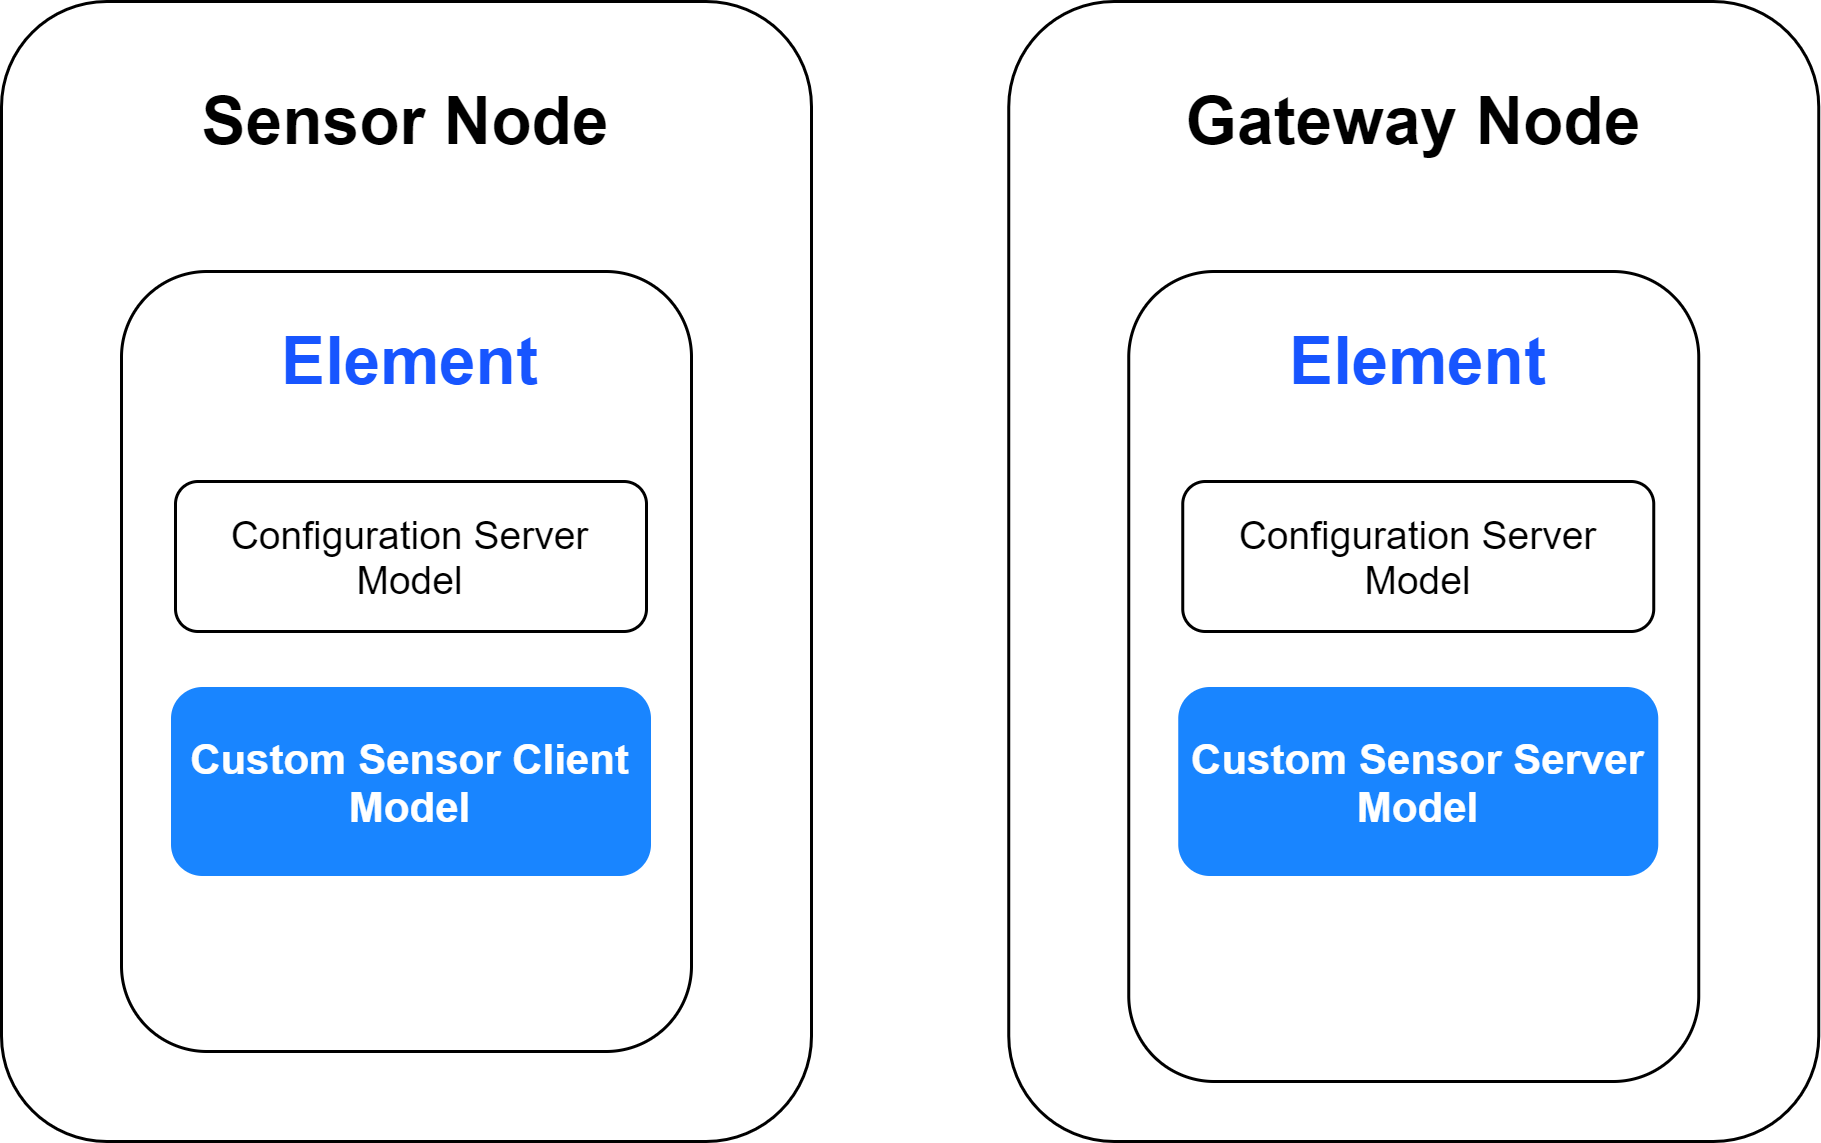
\includegraphics[scale=0.22]{mesh-node-architecture.png}
	\caption{Composição lógica dos nós da rede BLE Mesh}
	\label{fig:mesh-node-architecture}
\end{figure}

Os dispositivos foram organizados de acordo com o modelo \textit{Publish/Subscribe}, no qual os \textit{Sensor Nodes}, que possuem o Modelo Cliente, publicam mensagens do tipo SET sempre no mesmo grupo, de endereço 0xC100, em que o \textit{Gateway Node}, com o Modelo Servidor, está inscrito e recebe esses dados publicados, alterando seu estado. O conteúdo das mensagens enviadas é referente às medições dos sensores e, eventualmente, o resultado das perguntas da rotina de \textit{feedback}, realizados por cada nó da rede. Ao receber uma mensagem nova, o dispositivo central atualiza seu estado e coloca essa mensagem numa fila sincronizada, que será lida e processada por outra parte do programa principal do dispositivo. 

\begin{figure}[h!]
	\centering
	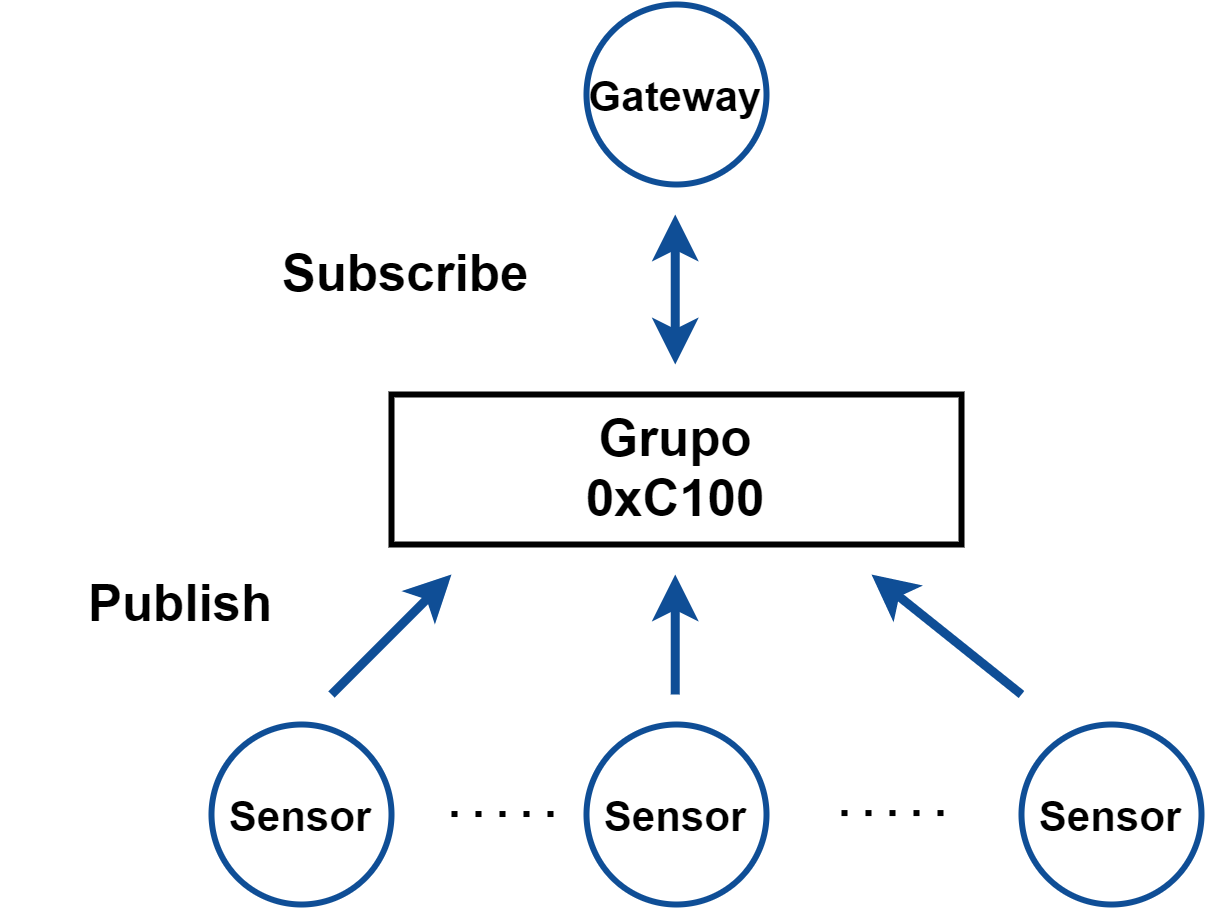
\includegraphics[scale=0.22]{ble-mesh-architecture.png}
	\caption{Arquitetura lógica da rede BLE Mesh}
	\label{fig:mesh-network-architecture}
\end{figure}

Essa fila sincronizada é a parte principal do dispositivo central, já que nela serão colocadas todas as mensagens recebidas dos nós da rede. Como citado na apresentação da estrutura de dados principal do Modelo, toda mensagem possui o nome do dispositivo que a enviou no início, antes dos dados dos sensores, sendo assim possível a identificação da mensagem em si após a sua retirada da fila e interpretação pelo programa principal.


\subsubsection{Wi-Fi} \label{dev-Wi-Fi}

A conexão do dispositivo gateway com a plataforma em nuvem é realizada utilizando o protocolo Wi-Fi. O ESP-IDF possui uma API pronta para ser utilizada para conectar o microcrontolador a um ponto de acesso Wi-Fi à escolha do usuário. Para isso, é necessário informar o SSID do ponto de acesso e a sua senha para conexão, armazenados em duas constantes no firmware. Definidas essas constantes, basta chamar a função de conexão fornecida pela API, que usará os valores definidos para realizar a conexão, bloqueando todo o programa até que a conexão seja estabelecida, obtendo endereços IPv4 e IPv6 (caso o ambiente de conexão seja capaz de fornecer os dois tipos de endereço para o dispositivo).

Com uma conexão com a Internet estabelecida, é necessário agora inicializar o dispositivo como um cliente MQTT e conectá-lo com o \textit{MQTT Broker} hospedado remotamente. Do mesmo modo, o ESP-IDF possui uma API que implementa as funcionalidades do protocolo MQTT utilizando conexão via TCP, para o qual é necessário informar o URL do \textit{MQTT Broker} a ser conectado, além dos valores de usuário e senha para autenticação no mesmo. Esses valores são salvos em uma estrutura no firmware, utilizada por uma função para inicializar o dispositivo como um cliente e estabelecer a conexão, a qual exige que haja uma conexão com a internet previamente estabelecida, como detalhado anteriormente. Se a conexão com o \textit{MQTT Broker} for realizada com sucesso, um evento indicando essa conexão será recebido pelo dispositivo, que estará pronto para enviar e receber mensagens.

O dispositivo gateway publicará as mensagens em tópicos referentes a cada dispositivo da rede, ou seja, cada dispositivo terá um tópico referente aos seus dados, seguindo o formato \texttt{devices\char`/device\char`_name}, no qual \textit{device\_name} se refere ao nome do dispositivo definido na estrutura de dados do \textit{Custom Sensor Model}, descrita na seção \ref{dev-bluetooth-section}. O conteúdo das mensagens enviadas nos tópicos se refere às leituras dos diferentes sensores, tanto as recebidas via BLE Mesh quanto as leituras do próprio dispositivo gateway.

Durante uma rotina de envio de dados ao servidor, o dispositivo publica cinco mensagens em seguida no mesmo tópico, sendo essas mensagens atreladas sempre ao mesmo dispositivo. Cada uma das mensagens contém dados de um dos sensores, ou seja, teremos uma mensagem com valores de temperatura e umidade do BME280, uma com valores de TVOC e $CO_{2}$ do SGP30, uma com valores das 6 cores e a intensidade da luz do ambiente do AS7262 e uma com o valor de ruído ambiente captado pelo microfone, além de uma última mensagem com as respostas de \textit{feedback} do usuário. Essa rotina de envio acontece toda vez que o dispositivo \textit{gateway} recebe dados via BLE Mesh ou quando uma medição dos seus próprios sensores é realizada. Todas essas mensagens seguem o formato a seguir, no qual \textbf{device\_name} se refere ao nome do dispositivo ao qual essa medição pertence, \textbf{sensor\_name} é o nome do sensor que realizou a medição e, por último, os valores de cada parâmetro lido:

\begin{align}
	\boldsymbol{device\_name},sensor="\boldsymbol{sensor\_name}", value1=v1,value2=v2 ... 
\end{align}

Este é o mesmo formato utilizado para inserir dados no InfluxDB, portanto enviá-los desta maneira para a plataforma facilita o seu tratamento posteriormente.


\section{Software}

O serviço de computação em nuvem escolhido para hospedar o banco de dados e a plataforma de visualização desse projeto foi o \textit{Amazon Web Services} (AWS). O AWS possui dezenas de serviços para diferentes aplicações, dos quais foi escolhido o \textit{Elastic Compute Cloud} (EC2), um serviço que permite que o usuário tenha uma máquina virtual com as características necessárias para hospedar as aplicações que desejar. O principal motivo que nos levou a escolher esse serviço de computação em nuvem foi o seu nível gratuito que, no caso do EC2, permite a configuração de uma máquina Linux do tipo \textit{t2.micro} \cite{aws-ec2-t2}, a qual optamos pela distribuição Ubuntu 20.04, com 1 GiB de memória RAM e 8 GiB de armazenamento SSD e que pode ser utilizada pelo período de 1 ano sem cobranças, que é o necessário para a realização do protótipo do projeto. Ao configurar a máquina pelo portal do AWS EC2, é fornecida uma chave criptografada do tipo \textit{Privacy-Enhanced Mail} (PEM) \cite{rfc1424}, utilizada para autenticar o acesso à máquina virtual através do protocolo SSH por um terminal externo, sendo essa a única forma de acessá-la. 

Com acesso ao sistema da máquina virtual, podemos fazer a instalação e configuração dos serviços a serem utilizados. Todos eles possuem suporte integral ao sistema operacional escolhido, o que torna o processo de instalação muito simples, bastando apenas seguir as respectivas documentações oficiais. 


\subsection{Eclipse Mosquitto}

A documentação de instalação do \textit{Eclipse Mosquitto} para Ubuntu pode ser encontrada na sua página oficial \cite{mosquitto}, que é bem simples, resumida nos seguintes comandos:

\begin{lstlisting}[language=bash, basicstyle=\ttfamily]
$ sudo apt-add-repository ppa:mosquitto-dev/mosquitto-ppa
$ sudo apt update
$ sudo apt install mosquitto
\end{lstlisting}

Após a instalação, o serviço é inicializado automaticamente, executado na porta TCP 1883 do sistema. Inicialmente, o \textit{broker} não possui nenhuma configuração de segurança, de modo que qualquer cliente que saiba o endereço de IP público da máquina consegue publicar mensagens. Para adicionar uma camada de segurança, é necessário criar um arquivo de texto em que cada linha segue o formato \texttt{usuário:senha} que serão aceitos pelo \textit{broker} como valores válidos para autenticação. Esse arquivo pode ser criptografado através do comando \texttt{mosquitto\char`_passwd -U arquivo\char`_de\char`_autenticacao} para que as senhas não fiquem salvas em texto puro. O caminho para esse arquivo de autenticação deve ser informado no arquivo de configuração geral do serviço, presente em \texttt{\char`/etc\char`/mosquitto\char`/conf.d\char`/config.conf}. Feito isso, os clientes precisam informar o par \textit{usuário:senha} para que consigam se conectar a esse \textit{broker}.

A comunicação é feita sobre o protocolo TCP sem nenhuma criptografia nas mensagens trocadas entre os dispositivos, de forma que as credenciais citadas anteriormente sejam transmitidas em texto e possam ser interceptadas e lidas por terceiros. Uma forma de melhorar ainda mais a segurança da conexão seria adicionar uma forma de criptografia na camada de transporte com o uso de SSL.

\subsection{InfluxDB}

Do mesmo modo que a aplicação anterior, a instalação do banco de dados InfluxDB ocorre de forma direta e simplificada, detalhada em sua página oficial \cite{influxdb-installation} e, após a instalação, a aplicação será executada por padrão na porta TCP 8086 do sistema. 

A interface de linha de comando da aplicação pode ser acessada através do comando \texttt{influx}, onde é possível realizar comandos e executar \textit{queries}, de acordo com a documentação oficial. A linguagem de interação com o banco de dados é chamada de \textit{InfluxQL}, muito parecida com a linguagem SQL. A primeira coisa a ser feita é criar um novo banco de dados utilizando o comando \texttt{CREATE DATABASE prototipo\char`_v1}, utilizado para salvar os dados desse projeto. Para criar usuários para que outras aplicações consigam acessar o banco de dados, usamos o comando \texttt{CREATE USER <username> WITH PASSWORD '<password>'} e criaremos dois usuários de acesso: 'telegraf' e 'grafana', sendo que o primeiro possui acesso total ao banco de dados (leitura e escrita), já que ele será responsável por escrever os dados recebidos da rede de sensores, e o segundo com permissões apenas de leitura. 

Todos os pontos inseridos no banco de dados possuem um \textit{timestamp} atrelado a eles, no formato UTC definido no RFC3339 \cite{rfc3339}, que indica o momento em que o ponto foi salvo. Os valores que se referem aos dados armazenados de fato são chamados de \textit{\textbf{Field Values}}, que podem ser números inteiros, valores booleanos, \textit{strings} ou de ponto flutuante. Esses dados podem ser identificados através de outros valores, chamados de \textit{\textbf{Field Keys}}, que servem para identificar o dado salvo, ou seja, age como o nome da variável, enquanto o valor anterior age como o conteúdo de fato da variável salva.

Outro par de campos que servem para descrever o dado salvo é \textit{\textbf{Tag Keys}} e \textit{\textbf{Tag Values}}, ambos do tipo \textit{string}, muito úteis quando é preciso buscar e agrupar dados. Todos esses campos citados são salvos dentro de um grupo chamado de \textit{\textbf{Measurement}}, sendo que o nome desse grupo descreve todos os dados que estão contidos dentro dele.

Finalmente, uma \textbf{série temporal} é o conjunto de pontos que conta com os mesmos valores de \textit{Measurement}, \textit{Tag} e \textit{Field Key}, com seus valores únicos identificados pelo \textit{Field Value} em conjunto com o \textit{timestamp}.

No contexto desse projeto, temos \textit{Measurements} que separam cada dispostivo único na rede, como mostrado na tabela \ref{table:measurements}, \textit{Tag Key} como sendo o nome de um dos quatro sensores únicos em um dispositivo ou \textit{feedback} e \textit{Field Key} os nomes dos diferentes parâmetros lidos, conforme a tabela \ref{table:tag-field-keys}.


\begin{table}[h!]
	\centering
	\begin{tabular}{|c|c|}
	\hline
	\textbf{Dispositivo} & \textit{\textbf{Measurement}}  \\ \hline
	Gateway              & esp\_1                         \\ \hline
	Nó 1                 & esp\_2                         \\ \hline
	Nó 2                 & esp\_3                         \\ \hline 
	\end{tabular}
	\caption{\textit{Measurements} presentes no banco de dados}
	\label{table:measurements}
\end{table}

\begin{table}[h!]
	\centering
	\begin{tabular}{|c|c|c|}
		\hline
		\textbf{Sensor} & \textit{\textbf{Tag Key}} & \textit{\textbf{Field Key}} \\ \hline
		BME280          & Temperature               & temperature, humidity       \\ \hline
		SGP30           & Air                       & eco2, tvoc                  \\ \hline
		AS7262          & Color                     & v, b, g, y, o, r, lux       \\ \hline
		Microfone       & Noise                     & noise\_level                \\ \hline
	\end{tabular}
	\caption{\textit{Tag Keys} e \textit{Field Keys} que identificam cada tipo de sensor e dados coletados}
	\label{table:tag-field-keys}
\end{table}

Ao final da seção \ref{dev-Wi-Fi}, foi explicado que os dados eram publicados seguindo um formato que facilitaria o tratamento e sua inserção no banco de dados. De fato, esse formato segue exatamente o que foi explicado agora, com cada campo correspondendo a sua respectiva função conforme as atribuições anteriores. A separação dos campos ocorre da seguinte forma:

\begin{center}
	$\underbrace{device\_name}_\text{Measurement},\underbrace{sensor=``sensor\_name``}_\text{Tag Set},\underbrace{value1=v1,value2=v2}_\text{Field Set}...$
\end{center}

\subsection{Telegraf}

O Telegraf é a aplicação responsável por conectar o Mosquitto com o InfluxDB, se inscrevendo nos tópicos de dados enviados pelos dispositivos da rede e inserindo-os no banco de dados. Como mencionado anteriormente, essa aplicação também é desenvolvida pela \textit{Influxdata}, mesma empresa que mantém o InfluxDB, de modo que suas documentações são muito parecidas \cite{telegraf-installation}. Logo, sua instalação também ocorre de maneira direta no sistema operacional escolhido através de poucos comandos. 

Simplificadamente, esse programa tem como objetivo ligar diferentes fontes de dados a diferentes destinos através de plugins previamente desenvolvidos, bastando o usuário escolher quais utilizar. Esses plugins são separados em duas categorias principais, plugins de entrada (\textit{input plugins}) e de saída (\textit{output plugins}). No nosso caso, utilizamos o \textit{\textbf{MQTT Consumer Input Plugin}} como plugin de entrada e o \textit{\textbf{InfluxDB v1.x Output Plugin}} como saída. A configuração e escolha dos plugins utilizados é feita através de um arquivo de configuração presente no caminho \texttt{\char`/etc\char`/telegraf\char`/telegraf.conf}, no qual a atribuição de valores às diferentes configurações de cada plugin é feita, seguindo as respectivas documentações. 

O primeiro plugin tem a função de se conectar ao MQTT Broker e se inscrever nos tópicos em que são escritos os dados provenientes da rede de dispositivos, recebendo assim as mesagens publicadas referentes às diferentes medições de sensores e, como definido na seção \ref{dev-Wi-Fi}, os tópicos seguem o formato \texttt{devices\char`/device\char`_name}, com conteúdo das mensagens no formato definido pelo InfluxDB. Dessa forma, definimos as configurações desse plugin:

\begin{lstlisting}[basicstyle=\small]
	[[inputs.mqtt_consumer]]
		servers = ["tcp://localhost:1883"]
		topics = [ "devices/#" ]
		data_format = "influx"

		username = <username_broker> 
		password = <senha_broker>
\end{lstlisting}

A aplicação Mosquitto é executada no endereço \texttt{tcp://localhost:1883}, no qual o Telegraf se conecta utilizando o usuário e senha aqui configurados para autenticação, se inscrevendo nos tópicos que atendem o formato passado em \textit{topics}, esperando mensagens no formato \textit{influx}. 

Já o segundo plugin tem a função de inserir todos os dados coletados pelo Telegraf em um banco de dados no InfluxDB. Precisamos apenas configurar a conexão do plugin com o banco de dados desejado, porque os dados coletados já estão no formato requisitado para a inserção. A configuração desse plugin ocorre no mesmo arquivo do anterior, adicionando os seguintes campos:

\begin{lstlisting}[basicstyle=\small]
	[[outputs.influxdb]]
		urls = ["http://localhost:8086"]
		database = "prototipo_v1"
		username = "telegraf"
		password = <senha_influxdb>

		namepass = ["esp*"]
\end{lstlisting}

O Telegraf se conecta com o InfluxDB através do endereço \texttt{http://localhost:8086}, se autenticando no banco de dados indicado na variável \textit{database} utilizando o par usuário e senha fornecidos. Utilizamos a variável \textit{namepass}, que verifica quais dados possuem a expressão \texttt{"esp"} em seu início, com o propósito filtrar os dados que serão inseridos de fato por esse plugin no banco de dados. Essa expressão estará presente nas mensagens recebidas, pois os nomes dos dispositivos (\texttt{device\char`_name}) definidos no projeto são \texttt{esp\char`_1}, \texttt{esp\char`_2} e \texttt{esp\char`_3}, já que temos apenas 3 dispositivos protótipos, que indicará também o \textit{measurement} inserido no banco de dados. 

Feitas essas configurações, as mensagens publicadas pelos dispositivos nos tópicos citados serão encaminhadas para o Telegraf, que fará sua inserção no banco de dados. A partir desse ponto, os dados estarão prontos para serem acessados e analisados.

\subsection{Grafana}

A plataforma de visualização de dados também pode ser instalada facilmente através de poucos comandos seguindo a sua própria documentação, presente em \cite{grafana-installation}. Logo após a instalação, a aplicação será executada na porta 3000 do sistema por padrão. Ao acessá-la pela primeira vez através de um navegador web utilizando o IP da máquina e a porta 3000, o usuário é levado a uma página de \textit{login} para a definição da senha de acesso para o usuário administrador que, depois de definida, pode ser utilizada para acessar o ambiente do Grafana. 

A aplicação possui um menu lateral onde é possível acessar parâmetros de configuração geral. A primeira configuração realizada é a conexão com o banco de dados, escolhendo a opção \textit{Configuration} $\rightarrow$ \textit{Data Sources} no canto esquerdo, que levará a uma página onde pode ser escolhido o tipo da fonte de dados a ser conectado a partir de uma lista com inúmeras conexões possíveis, onde selecionamos o InfluxDB, e depois é necessário preencher as informações de conexão, análogas às que foram utilizadas pelo Telegraf, como ilustrado na figura \ref{fig:grafana-datasource}.

\begin{figure}[h!]
	\centering
	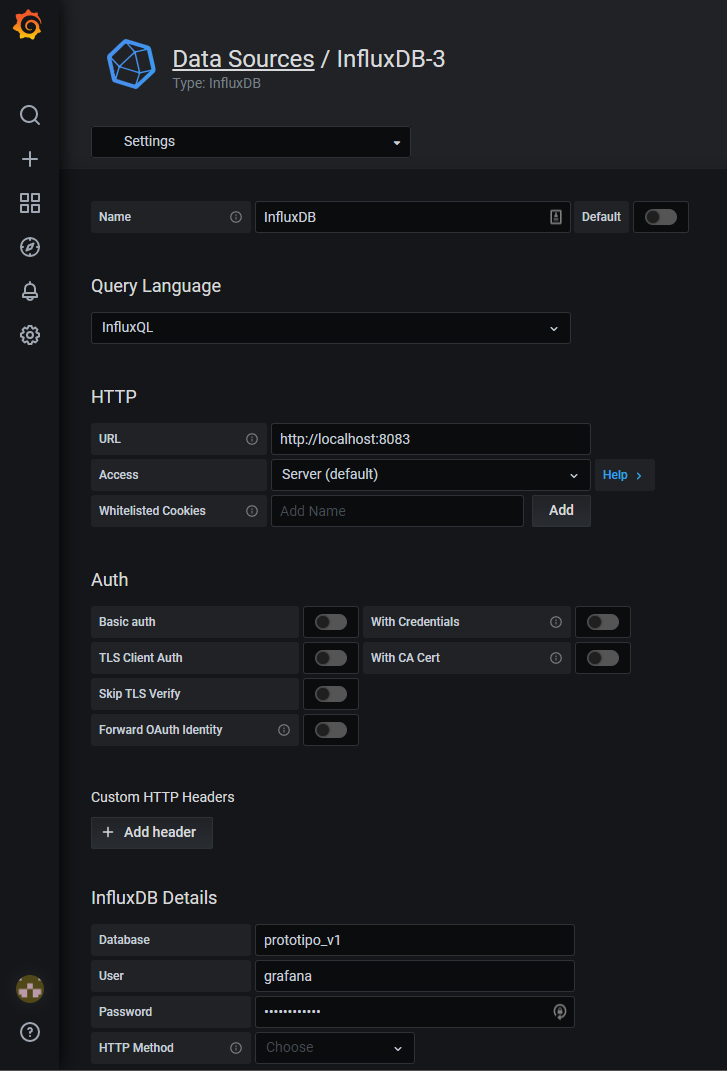
\includegraphics[scale=0.4]{grafana-datasource.png}
	\caption{Conexão do Grafana com a fonte de dados InfluxDB}
	\label{fig:grafana-datasource}
\end{figure}

O Grafana possui diferentes opções de painéis como tabelas, gráficos de linhas e de barras, destinados a mostrar dados acessados atavés de consultas específicas ao banco de dados. Essas consultas, normalmente, retornam partes de uma das séries temporais referentes a medições de sensores em um período de tempo específico, determindo por uma variavel presente no canto superior direito de todas as páginas do \textit{dashboard}, onde o usuário pode selecionar a faixa de tempo desejada. A figura \ref{fig:grafana-query} ilustra como uma consulta pode ser configurada dentro de um painel, exemplificando o caso de acesso à série temporal referente às medições de temperatura do dispositivo \textit{esp\_1} para serem visualizados em um gráfico de linha.

\begin{figure}[h!]
	\centering
	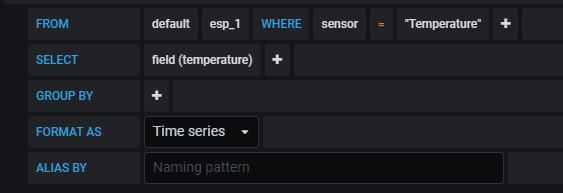
\includegraphics[scale=0.7]{grafana-graph-query.png}
	\caption{Exemplo de consulta feita em um painel do Grafana}
	\label{fig:grafana-query}
\end{figure}


A configuração de painéis gráficos também permite que sejam estabelecidos valores limiares para as séries temporais monitoradas e, a partir desses limiares, configurar alertas que podem ser notificados em diferentes serviços externos, dentre eles alguns serviços de comunicação como Slack, Telegram, Microsoft Teams e email. 

Os valores de limiar foram definidos com base nos níveis recomendados para cada indicador de qualidade e conforto medidos, discutidos na seção \ref{arte-indicadores}. O sistema de alertas foi configurado para avaliar a cada 10 minutos os últimos dados coletados e, se estiverem fora dos níveis recomendados, enviam notificações para um canal em um servidor do aplicativo Slack, para demonstrar um possível caso de uso em um escritório de uma empresa que faz uso desse meio de comunicação.

%! Precisamos incluir imagens e uma descrição do dashboard desenvolvido aqui ou só no capítulo de testes?


\subsection{Servidor}

Com objetivo de facilitar o acesso à plataforma de visualização, registramos o domínio \underline{coent.tech} gratuitamente por 1 ano através do programa dedicado a estudantes \textit{GitHub Education} \cite{github-education}. Como serviço de DNS, foi utilizado o \textit{Cloudflare} \cite{cloudflare}, redirecionando acessos ao domínio adquirido ao IP público da máquina virtual fornecido pela AWS.

Cada aplicação citada até aqui roda em um porta diferente no sistema, porém acessá-las externamente através dessas portas não é seguro nem prático. Dado isso, utilizamos o NGINX, uma aplicação que atua como \textit{reverse proxy}, ou seja, todas as requisições feitas ao nosso sistema passarão por essa aplicação, a qual redireciona as requisições para os serviços adequados. Deste modo, podemos deixar apenas as portas 80 (HTTP), 443 (HTTPS) e 1883 (MQTT/TCP) liberadas para aceitarem conexões externas e que serão monitoradas pelo NGINX.

As configurações de redirecionamento são definidas por regras presentes em um arquivo específico, onde são explicitados quais os destinos que devem receber as requisições, dependendo da URL de origem. Os valores escolhidos para os pares subdomíno - aplicação estão mostrados na tabela \ref{table:nginx-config}. Todos os subdomínios citados também foram adicionados às configurações do \textit{Cloudflare} para que a tradução dos nomes seja feita corretamente.

\begin{table}[h!]
	\centering
	\begin{tabular}{|c|c|}
	\hline
	\textbf{Subdomínio}         & \textbf{Aplicação Local}                                               \\ \hline
	mosquitto.coenv.tech & \begin{tabular}[c]{@{}c@{}}Eclipse Mosquitto\\ porta 1883\end{tabular} \\ \hline
	dashboard.coenv.tech & \begin{tabular}[c]{@{}c@{}}Grafana\\ porta 3000\end{tabular}           \\ \hline
	coenv.tech           & Página HTML estática                                                   \\ \hline
	\end{tabular}
	\caption{Tabela de redirecionamento configurada para o NGINX}
	\label{table:nginx-config}
\end{table}

Visando adicionar uma camada maior de segurança, utilizamos o \textit{certbot}, um programa desenvolvido pela \textit{Electronic Frontier Foundation} que facilita a adoção de certificados SSL emitidos gratuitamente pela \textit{Let's Encrypt} \cite{certbot}\cite{lets-encrypt}, para adicionar um certificado no nosso servidor e permitir conexões seguras via HTTPS. 

Portanto, temos as seguintes formas de acessar os serviços disponibilizados pelo servidor:

\begin{itemize}
	\item Acesso ao Mosquitto MQTT Broker: \underline{mqtt://mosquitto.coenv.tech/}
	\item Acesso à plataforma de visualização de dados: \underline{https://dashboard.coenv.tech/}
	\item Acesso à página web com informações sobre o projeto: \underline{https://coenv.tech/}
\end{itemize}


\begin{figure}[h!]
	\centering
	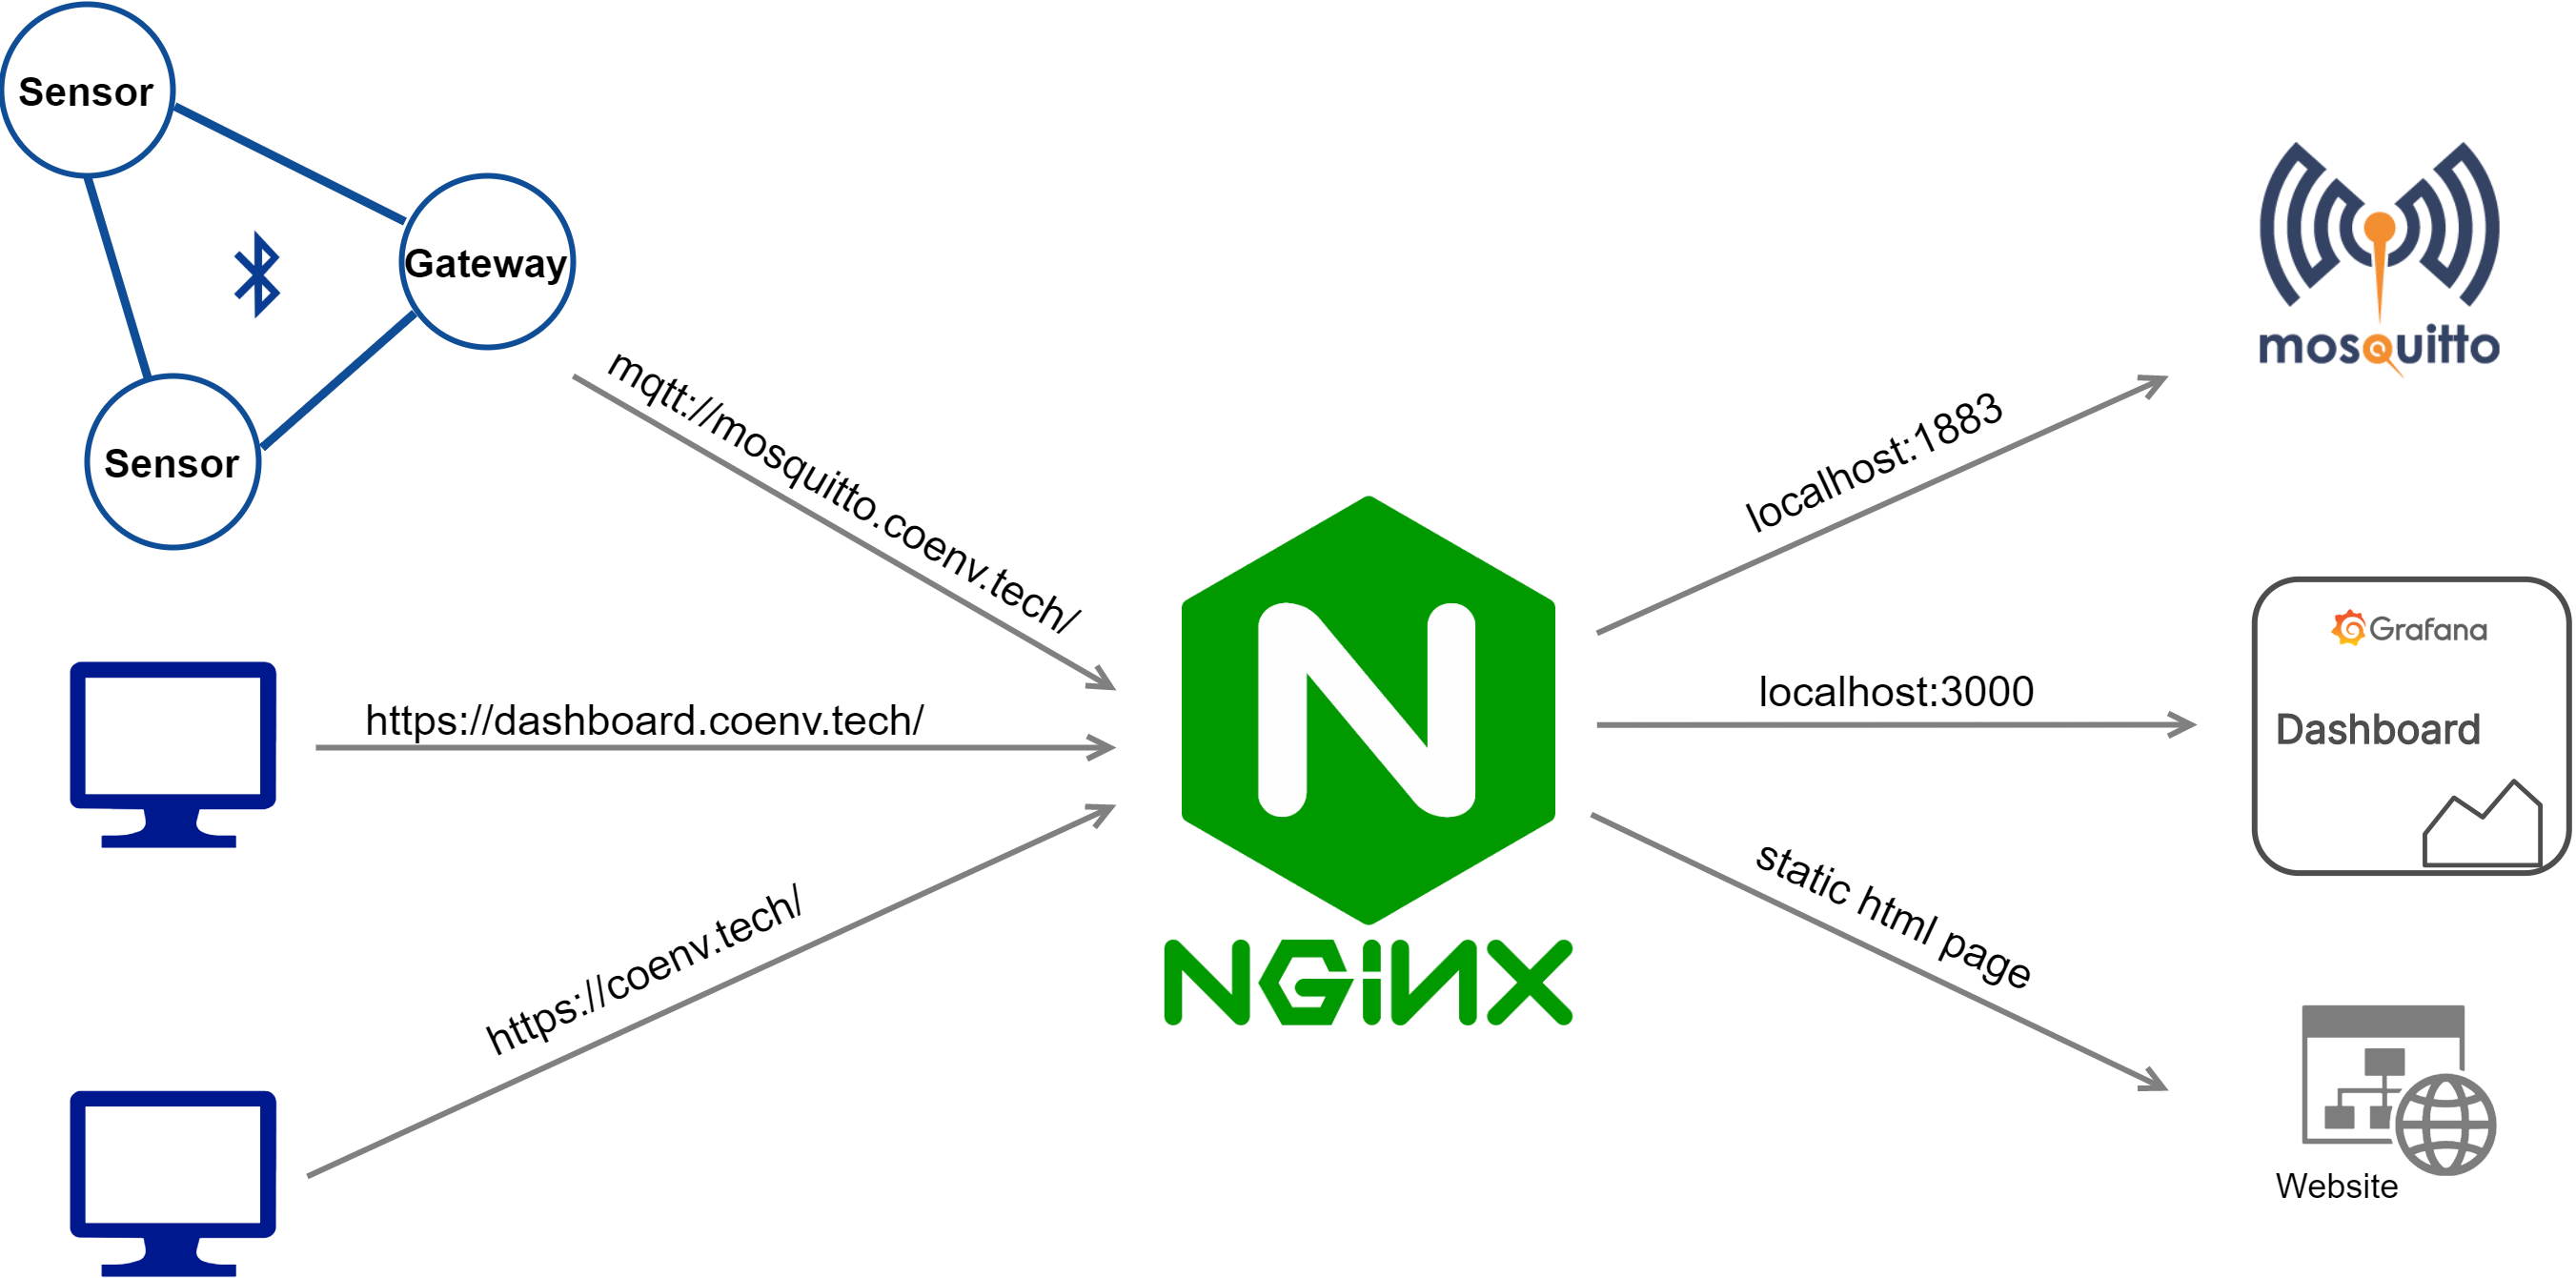
\includegraphics[scale=0.16]{server-architecture.png}
	\caption{Arquitetura do servidor em nuvem}
	\label{fig:cloud-server-architecture}
\end{figure}

\section{Mecânica}

Foi projetado um case mecânico para proteger a eletrônica dos dispositivos, a ser impresso em 3D. 

O case é composto por duas peças, uma base, onde fica fixada a placa, e uma tampa onde ficam fixados o display OLED e os botões. As laterais abertas permitem que sejam feitos ajustes dos módulos com sensores sem afetar o funcionamento destes. 

\begin{figure}[h]
\centering
	\begin{subfigure}{0.5\textwidth}
		\centering
		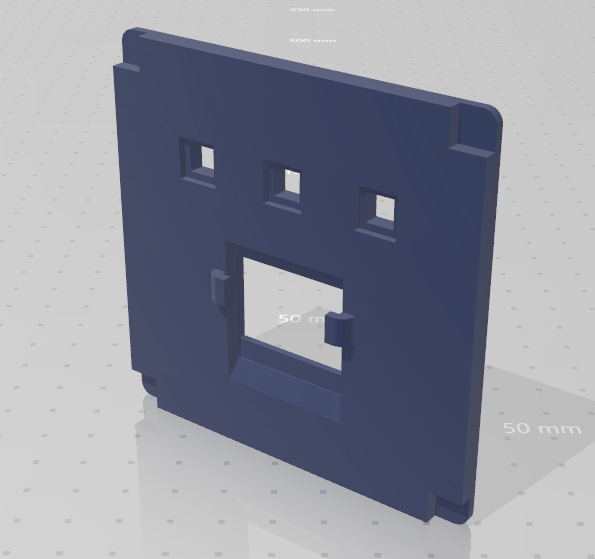
\includegraphics[width=0.9\textwidth]{mec-tampa.jpeg}
		\caption{Tampa}
		\label{fig:tampa-mec}
	\end{subfigure}%
	\begin{subfigure}{0.5\textwidth}
		\centering
		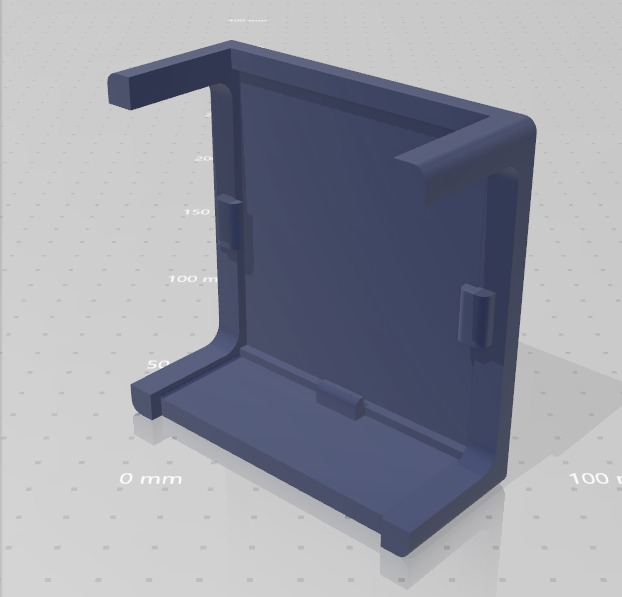
\includegraphics[width=0.9\textwidth]{mec-base.jpeg}
		\caption{Base}
		\label{fig:base-mec}
	\end{subfigure}
	\caption{Case Mecânico}
	\label{fig:mecanicas}
\end{figure}

\section{Custos}

\begin{tabular}{ |p{4.5cm}|p{2cm}|p{3cm}|p{3cm}|  }
	\hline
	\multicolumn{4}{|c|}{Hardware} \\
	\hline
	\hline
	Componente & Quantidade & Custo Unit. & Total\\
	\hline
	ESP32 DevKitC & 3 & R\$ & R\$ \\
	BME280 & 3 & R\$35,30 & R\$105,80 \\
	SGP30 & 3 & R\$ & R\$ \\
	AS7262 & 3 & R\$ & R\$ \\
	Microfone MAX4466 & 3 & R\$33,06 & R\$99,18 \\
	LCD Oled SSD1306 & 3 & R\$28,88 & R\$86,64 \\
	Botões Push-Button & 9 & R\$0,37 & R\$3,33 \\
	Capacitor 220nF & 9 & R\$0,10 & R\$0,90 \\
	Resistor 1kOhm & 9 & R\$0,10 & R\$0,90 \\
	Cabos USB micro & 3 & R\$9,90 & R\$29,7 \\
	\hline
	\multicolumn{2}{|c|}{ } & Total & R\$326,45 \\
	\hline
\end{tabular}

Licença Altium 
3x Placa fibra de vidro face simples 7x7cm R\$11,00
Cabos R\$19,45
Fresa CNC pode ter custo adicional
Impressora 3D 

\end{document}
